%! Author = metametamoon
%! Date = 1/27/25

% Preamble
\documentclass[11pt]{article}

\usepackage{listings}
\usepackage{xcolor}

\definecolor{codegreen}{rgb}{0,0.6,0}
\definecolor{codegray}{rgb}{0.5,0.5,0.5}
\definecolor{codepurple}{rgb}{0.58,0,0.82}
\definecolor{backcolour}{rgb}{0.95,0.95,0.92}

\lstdefinestyle{mystyle}{
    backgroundcolor=\color{backcolour},
    commentstyle=\color{codegreen},
    keywordstyle=\color{magenta},
    numberstyle=\tiny\color{codegray},
    stringstyle=\color{codepurple},
    basicstyle=\ttfamily\footnotesize,
    breakatwhitespace=false,
    breaklines=true,
    captionpos=b,
    keepspaces=true,
    numbers=left,
    numbersep=5pt,
    showspaces=false,
    showstringspaces=false,
    showtabs=false,
    tabsize=2
}

\lstset{style=mystyle}


% Packages
\usepackage{amsmath}
\usepackage[utf8]{inputenc}
\usepackage[russian]{babel}
\usepackage{amsfonts}
\usepackage{amssymb}
\usepackage{graphicx}
\usepackage{subcaption}
\usepackage{caption}

\newcommand{\realpositive}{\mathbb{R}_{\geqslant 0}}
\DeclareMathOperator*{\argmin}{arg\,min}
\newcommand{\dstarlite}{\(D^*\ lite\)\,}
\newcommand{\astar}{\(A^*\)\,}

% Document
\begin{document}
    \title{LPA$^*$ и D$^*$ lite}
    \author{Лев Сорвин, Максим Хабаров \\ под руководством Константина Яковлева}
    \date{2025-01-29}
    \maketitle


    \section{Мотивация}
    Во многих областях искусственного интеллекта естественным образом появляется планирования путей на больших графах.
    Большая часть исследований в этой задаче покрывает задачу в случае, когда граф нам целиком известен заранее.
    Однако многим системам приходится сталкиваться с динамическими изменениями в графе и приходиться адаптироваться к изменившимся условиям, поскольку предыдущий итог планирования может потерять актуальность


    \section{Постановка задачи}
    Пусть нам дан граф $G = (V, E)$, где $V$ --- конечное множество вершин, $E \subset V \times V \times \realpositive$ --- множество взвешенных ребер.
    При этом будем считать, что в графе нет кратных ребер, ввиду чего можно ввести функцию веса ребра $w: V \times V \rightarrow {\realpositive \lor \infty}$
    Путем в графе будем называть конечную последовательность $A = [v_1, v_2, \dots, v_n]$ такую, что для каждого $i = 1, \dots, n-1$: $w(v_i, v_{i+1}) \neq \infty$.
    Множество конечных последовательностей вершин мы будем обозначать $P = P(V)$.
    Весом пути мы будем называть выражение $w(A) = \sum_{i = 1}^{n-1} w(v_i, v_{i+1})$.
    Началом пути мы будем называть при этом первый элемент последовательности и обозначать $s(A)$, а концом пути --- последний элемент последовательности, и обозначать $d(A)$.

    Мы хотим решать задачу минимального пути --- нам даны вершины $s, d \in V$  (далее мы считаем, что $s, d, V$ фиксированы) и мы должны найти
    $$A_{plan}= \argmin_{\substack{A \subset V \text{ --- путь в } G \\ s(A) = s \\ d(A) = d}} w(A).$$
    Мы будем также говорить тогда, что $A = \mathtt{optpath}(G, s, d)$.

%    \pagebreak
    \newcommand{\fplan}{\mathtt{plan}}
    \newcommand{\fextract}{\mathtt{extract}}
    \newcommand{\fempty}{\mathtt{empty}}
    Сформулируем более точно алгоритмическую задачу.
    На $i$-ом шаге мы получаем информацию $E_i \subset V \times V \times \realpositive \lor \infty$ об изменении весов ребер в графе.
    Тогда \textit{алгоритмом для решения задачи долгосрочного планирования} мы будем называть тройку $(T, \fplan, \fextract)$ из произвольного множества и двух вычислимых фукнций соответственно, такую что:
    \begin{align*}
        &\fempty \in T \\
        &\fplan: E \times T \rightarrow T \\
        &\fextract: T \rightarrow P(V) \\
        &\fextract(\fplan(E, \fempty)) = \mathtt{optpath}(G, s, d) \\
        &\fextract(t_0) = \mathtt{optpath}((V, E'), s, d) \rightarrow \\
        &\qquad \fextract(\fplan(E_{new}, t_0)) = \mathtt{optpath}((V, E' \leftarrow E_{new}), s, d)
    \end{align*}

    Мы будем применять алгоритм в следующем коде (который следует рассматривать как синтаксический сахар над машиной Тьюринга):
    \begin{verbatim}
active_plan = empty
for i in 1..n:
     e_new_i = get_e_new_i()
     active_plan = plan(e_new_i, active_plan)
     shortest_path = extract(active_plan)
    \end{verbatim}
    Мы хотим минимизировать число итераций алгоритма $\fplan$ и $\fextract$ в ходе исполнения псевдокода выше.


    \section{Метод решения}

    Несложно заметить, что реализация функции \(\fplan\), которая заново находит кратчайший путь в графе с обновленными ребрами, является решением нашей задачи.
    Однако оптимальность этого решения оставляет желать лучшего: даже при небольших изменениях ребер в графе нам придется выполнять заново всю процедуру планирования.
    В связи с этим хочется использовать \textit{инкрементальные}, которые во время планирования сохраняют полезную в дальнейшем информацию, чтобы ее затем эффективно переиспользовать в новой задаче планирования.
    Такие алгоритмы уже есть --- например, Dynamic SWSF-FP~\cite{RAMALINGAM1996267}.

    С другой стороны, использование эвристик в задачах поиска дает на практике очень существенное преимущество, в связи с чем широко используется.
    Наиболее популярным алгоритмом для задачи планирования с использованием эвристик является алгоритм $A^*$~\cite{Nilsson1971ProblemsolvingMI}.
    Однако алгоритм $A^*$ сам по себе не является инкрементальным в связи с чем его использование в нашей задаче приведет к повторному планированию крайне часто.

    Мы хотим объединить эти два подхода --- использовать эвристики для направления поиска и использовать инкрементальность для оптимального пересчета решения при появлении новых данных.
    Для этого мы переиспользуем идею из алгоритма Dynamic SWSF-FP.
    Как мы знаем, уравнение \[ g^*(v) = \begin{cases}
                                            0 &  v = s\\
                                            \min_{v' \in neighbors(v)} (w(v, v') + g^*(v')) \\
    \end{cases} \]
    задает оценку $g^*(v)$ кратчайшего пути от $s$ до произвольной вершины $v$.
    Мы будем для каждой вершины поддерживать оценку веса кратчайшего пути $g$ в том же значении, как и в алгоритме $A^*$, а также
    величину \[rhs(v) = \min_{v' \in neighbors(v)} (w(v, v') + g(v')). \]
    Несложно заметить, что если во всех вершинах $rhs(v) = g(v)$, то $g(v) = g^*(v)$ для всех вершин $v$.
    Будем называть вершину $v$ \textit{неконсистентной}, если $rhs(v) \neq g(v)$.
    В ходе алгоритма мы будем итеративно исправлять неконсистентность, пока ее исправление может привести к нахождению кратчайшего пути.

    Заметим, что при изменении веса ребер у нас меняются $rhs$-значения у вершин, связанных с этими ребрами.
    По нашему алгоритму, мы будем исправлять неконсистентность лишь у необходимого количества вершин, начиная с вершин, находящихся рядом с измененными ребрами.


    \section{Алгоритм \dstarlite}
    Возможность пересчитывать кратчайшие пути позволяет нам решать следующую задачу.
    Пусть у нас есть агент с ограниченным зрением, который должен дойти до некоторой точки на карте.
    Изначально у него нет никакой карты местности, но он обновляет свои данные, когда препятствия попадают в его поле зрения.
    Агент всегда хочет идти по оптимальному пути к цели, но информация о препятствиях будет заставлять его перестраивать план.

    В этой ситуации можно использовать алгоритм $LPA^*$ следующим образом.
    Агент может на очередном шаге строить кратчайший путь от цели до себя, основываясь на известных ему данных.
    После очередного шага он использует информацию о полученных препятствиях, чтобы обновить план кратчайшего пути от цели до себя.

    \begin{figure}
        \begin{lstlisting}[language=Python, caption=D* lite ]
def CalculateKey(s):
     return (min(g(s), rhs(s) + h(s), min(g(s), rhs(s))))
def Initialize():
     U = dict()
     for s in S:
          rhs(s) = g(s) = infinity
     rhs(start) = 0
     U.insert((start, (h(start), 0)))

def UpdateVertex(u):
     if u != start:
          rhs(u) =min([g(v) + c(v, u) for v in pred(u)])
     if u in U:
          U.remove(u)
     if g(u) != rhs(u):
          U.insert(u, CalculateKey(u))

def ComputeShortestPath():
     while U.topKey() < CalculateKey(goal) or rhs(goal) != g(goal):
          u = U.pop()
          if g(u) > rhs(u):
               g(u) = rhs(u)
               for s in succ(u):
                    UpdateVertex(s)
          else:
               g(u) = infinity
               for s in succ(u) + {u}:
                    UpdateVertex(s)

def Main():
     Initialize()
     while True:
          ComputeShortestPath()
          // make move along the shortest path to goal
          for (u, v) in observedEdges:
               UpdateVertex(u)
               UpdateVertex(v)
        \end{lstlisting}
    \end{figure}


    \section{Экспериментальные исследования}

    Мы будем исследовать алгоритм \dstarlite в задаче поиска пути на карте с ограниченной видимостью.
    Для этого мы используем карты с датасета MovingAI~\cite{sturtevant2012benchmarks}.
    Мы используем 4 карты, которые обобщают реально встречающиеся топологии у агентов в реальной жизни: план этажа, город, разные виды лабиринтов (см. рис.  \ref{fig:maps}).
    Ширина каждой карты, кроме Labyrinth, примерно равна 250, ширина Labyrinth же примерно равна 800 (точные размеры карт доступны в репозитории).
    Здесь и далее, когда мы говорим о малой видимости, мы имеем в виду радиус видимости в 5 клетки, большой видимости --- в 50 клеток.
    \begin{figure}
        \centering
        \begin{subfigure}[b]{0.24\textwidth}
            \centering
            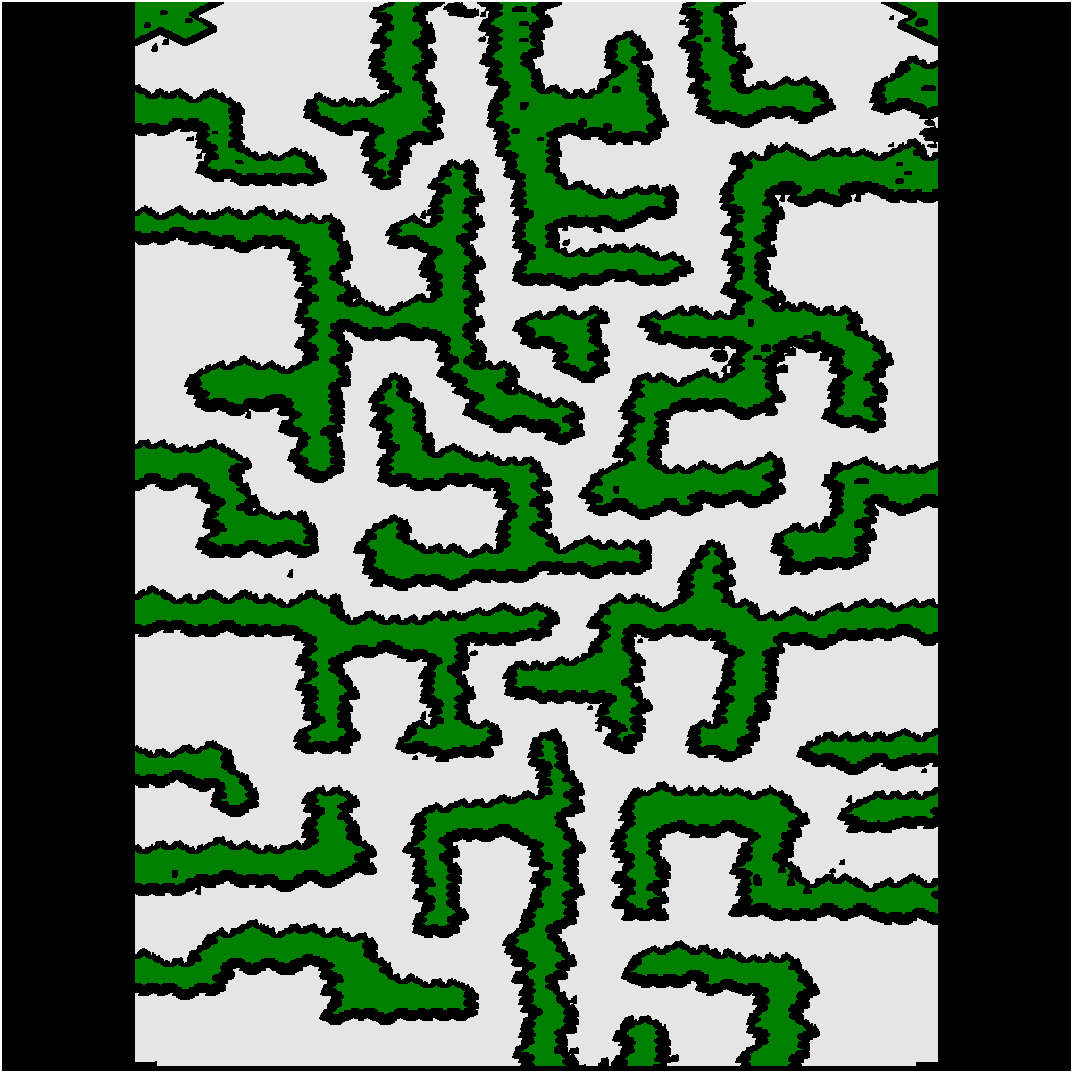
\includegraphics[width=\textwidth]{../maps/Labyrinth}
            \caption{Labyrinth}
            \label{fig:y equals x}
        \end{subfigure}
        \hfill
        \begin{subfigure}[b]{0.24\textwidth}
            \centering
            
\includegraphics[width=\textwidth]{../maps/den401d}
            \caption{den401d}
        \end{subfigure}
        \hfill
        \begin{subfigure}[b]{0.24\textwidth}
            \centering
            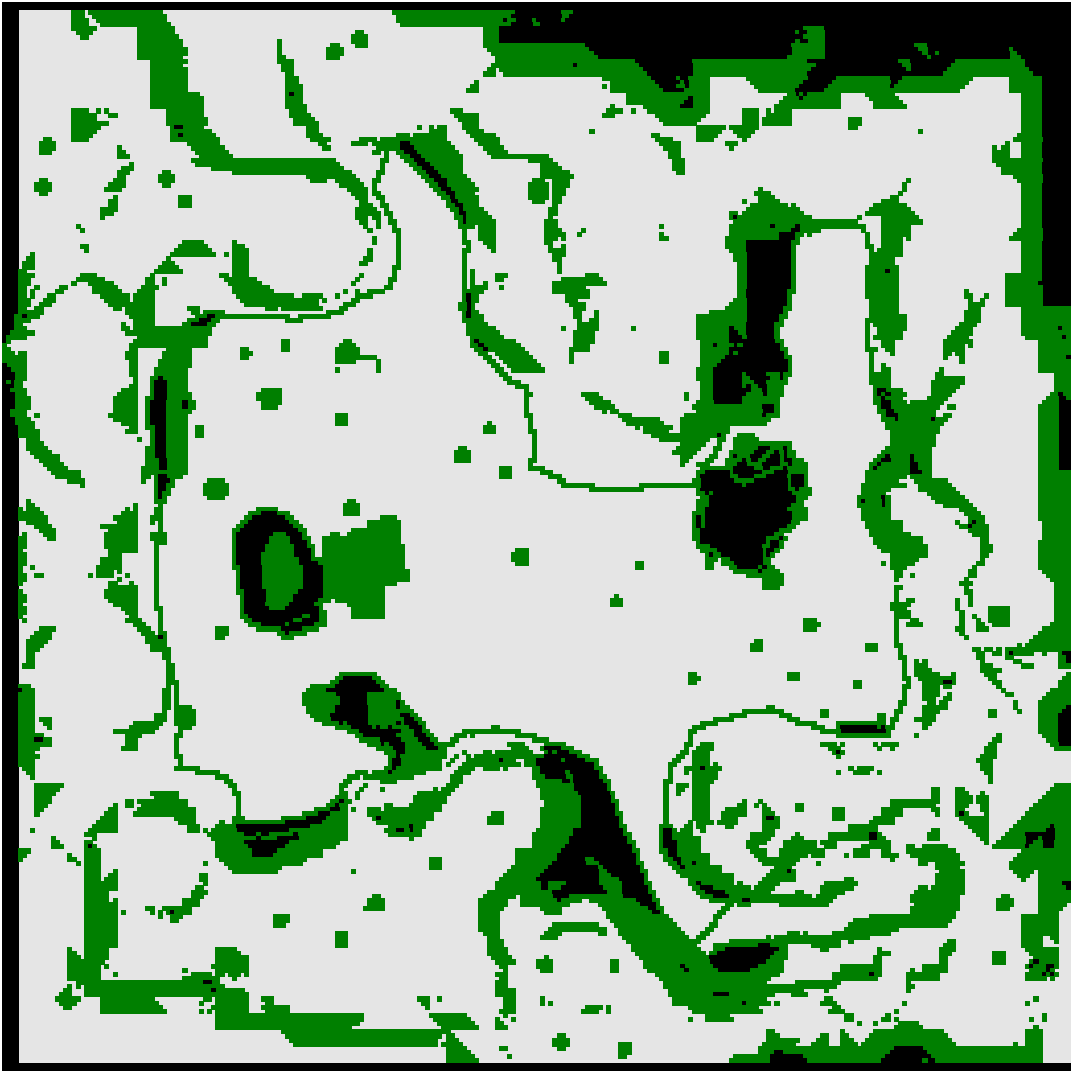
\includegraphics[width=\textwidth]{../maps/brc504d}
            \caption{brc504d}
        \end{subfigure}
        \begin{subfigure}[b]{0.24\textwidth}
            \centering
            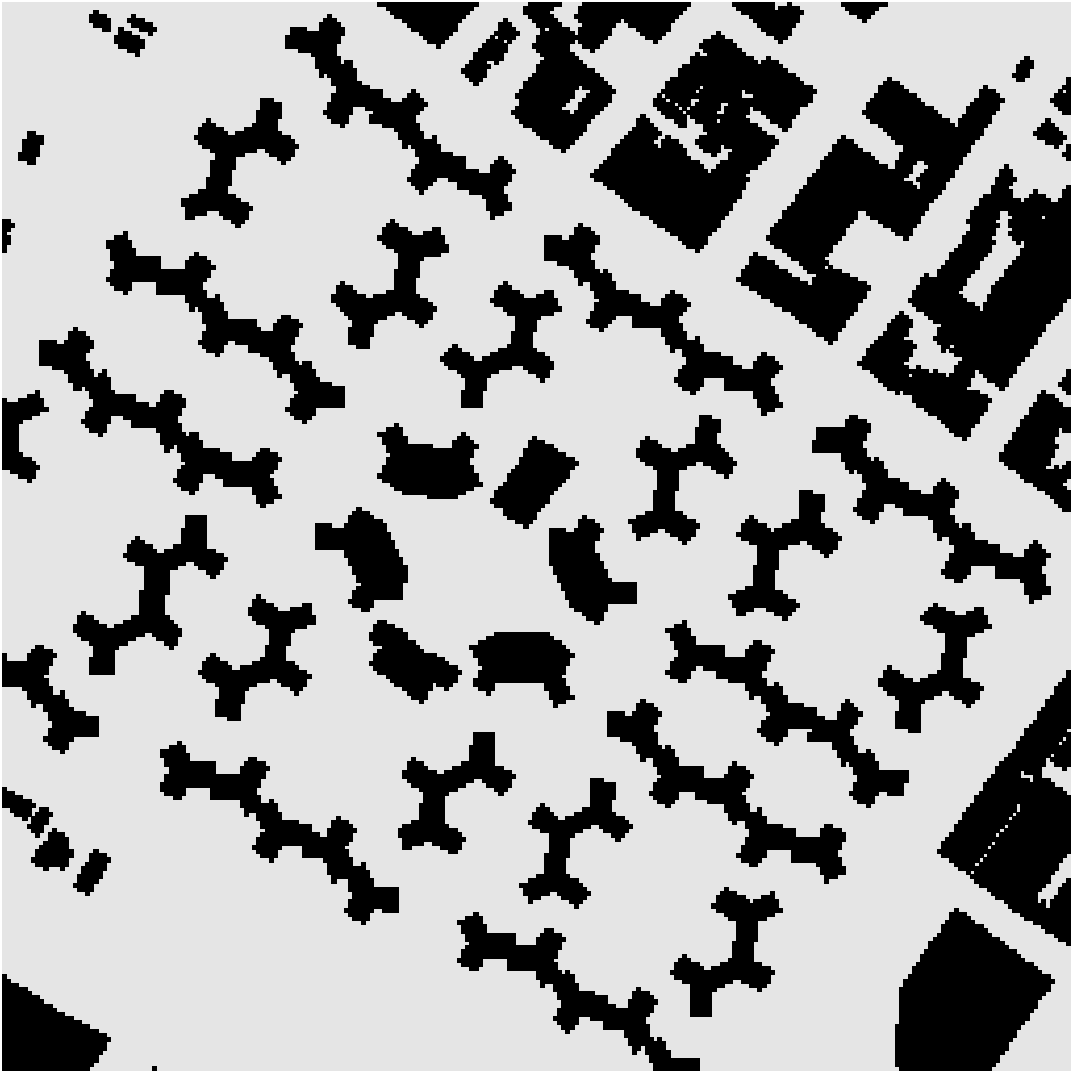
\includegraphics[width=\textwidth]{../maps/NewYork_1_256}
            \caption{NewYork}
        \end{subfigure}
        \caption{Карты, использующиеся для измерения производительности}
        \label{fig:maps}
    \end{figure}

    Для каждой карты мы равномерно выберем хотя бы 100 сценариев, выбирая каждый 5 сценарий в файле сценариев, и запустим на них агента с различными радиусами видимости.
    Будем отслеживать только производительность, считая, что память не является узким местом в областях применения данного алгоритма.
    В качестве метрик мы возьмем время работы алгоритма на карте, а также для воспроизводимости результатов число операций, модифицирующих очередь с приоритетом (во всех алгоритмах мы использовали для очереди с приоритетом одну и ту же структуру данных) и количество чтений/записей полей вершины.

    \begin{figure}
        \centering
        \begin{subfigure}[b]{0.48\textwidth}
            \centering
            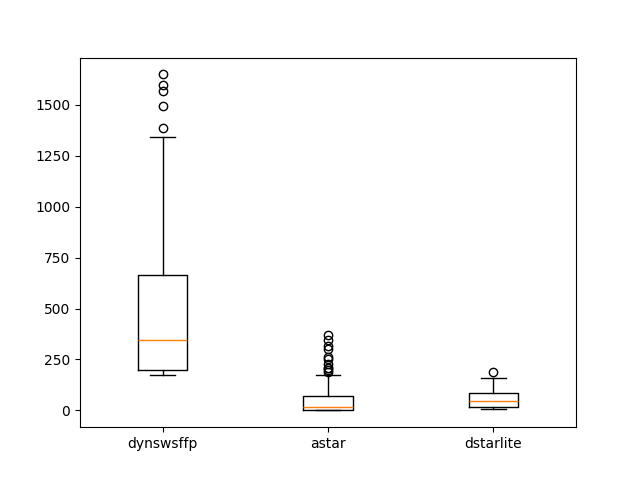
\includegraphics[width=\textwidth]{../plots/r5/den401d-('dynswsffp', 'astar', 'dstarlite').png}
        \end{subfigure}
        \hfill
        \begin{subfigure}[b]{0.48\textwidth}
            \centering
            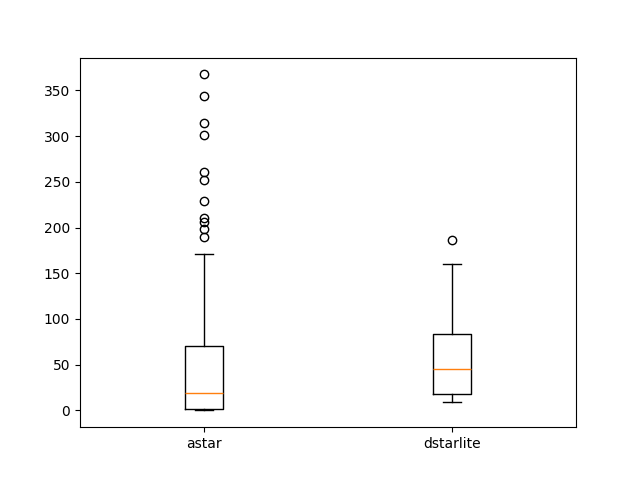
\includegraphics[width=\textwidth]{../plots/r5/den401d-('astar', 'dstarlite').png}
        \end{subfigure}
        \caption{den401d, малая видимость, производительность в ms}
        \label{fig: den401d-r5}
    \end{figure}

    \begin{figure}
        \centering
        \begin{subfigure}[b]{0.48\textwidth}
            \centering
            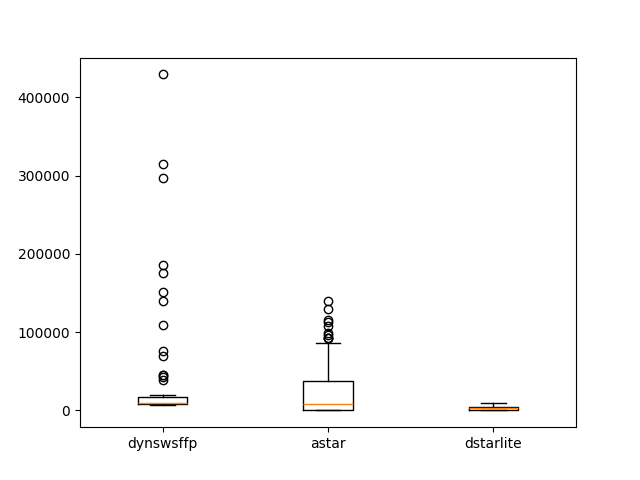
\includegraphics[width=\textwidth]{../plots/r5/Labyrinth-('dynswsffp', 'astar', 'dstarlite').png}
        \end{subfigure}
        \hfill
        \begin{subfigure}[b]{0.48\textwidth}
            \centering
            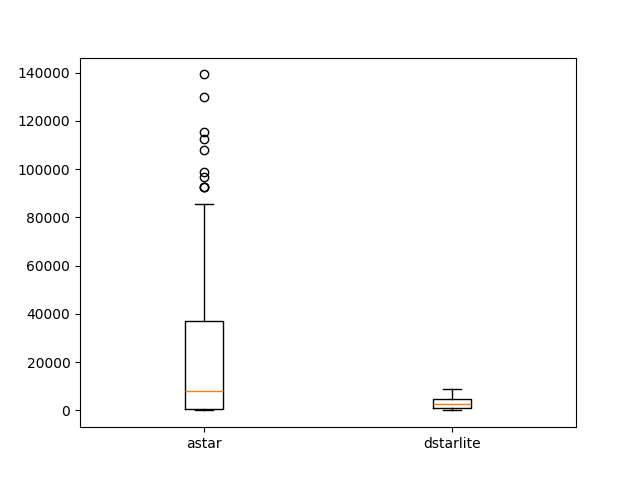
\includegraphics[width=\textwidth]{../plots/r5/Labyrinth-('astar', 'dstarlite').png}
        \end{subfigure}
        \caption{Labyrinth, малая видимость, производительность в ms}
        \label{fig: Labyrinth-r5}
    \end{figure}

    \begin{figure}
        \centering
        \begin{subfigure}[b]{0.48\textwidth}
            \centering
            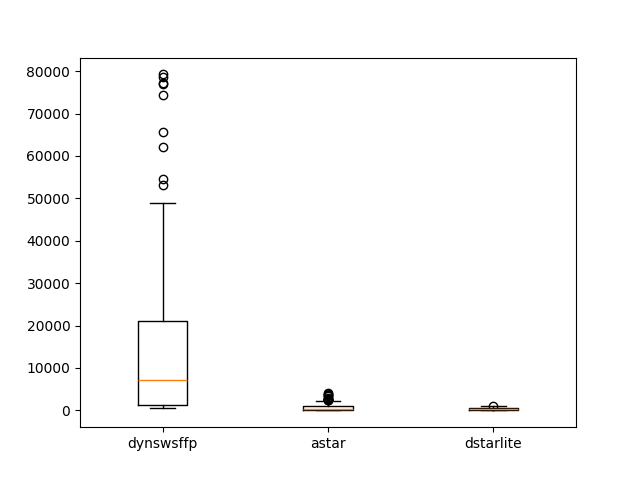
\includegraphics[width=\textwidth]{../plots/r5/brc504d-('dynswsffp', 'astar', 'dstarlite').png}
        \end{subfigure}
        \hfill
        \begin{subfigure}[b]{0.48\textwidth}
            \centering
            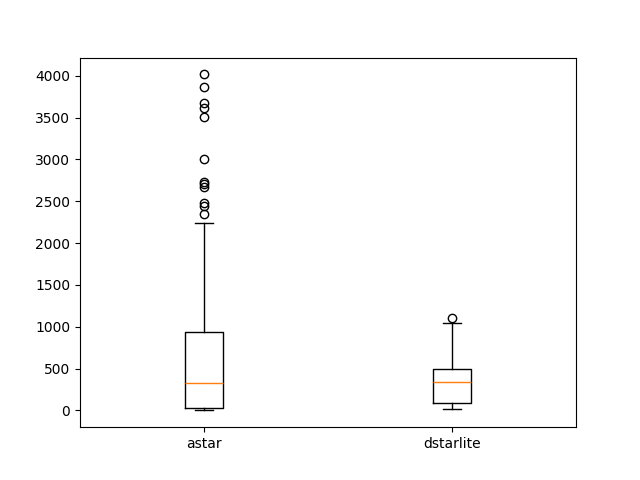
\includegraphics[width=\textwidth]{../plots/r5/brc504d-('astar', 'dstarlite').png}
        \end{subfigure}
        \caption{brc504d, малая видимость, производительность в ms}
        \label{fig: brc504d-r5}

    \end{figure}

    \begin{figure}
        \centering
        \begin{subfigure}[b]{0.48\textwidth}
            \centering
            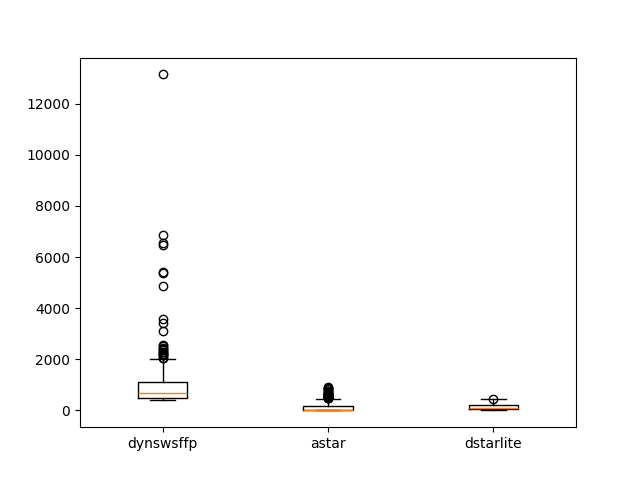
\includegraphics[width=\textwidth]{../plots/r5/NewYork_1_256-('dynswsffp', 'astar', 'dstarlite').png}
        \end{subfigure}
        \hfill
        \begin{subfigure}[b]{0.48\textwidth}
            \centering
            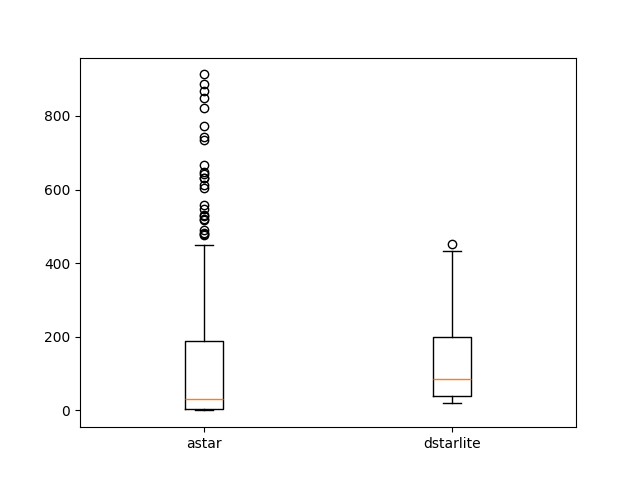
\includegraphics[width=\textwidth]{../plots/r5/NewYork_1_256-('astar', 'dstarlite').png}
        \end{subfigure}
        \caption{NewYork\_1\_256, малая видимость, производительность в ms}
        \label{fig: NewYork_1_256-r5}
    \end{figure}



    Во-первых, результаты экспериментов показали, что использование эвристик дает крайне существенный прирост к производительности, в связи с чем нерационально использовать инкрементальность алгоритма вместо использования эвристик.

    Во-вторых, на низкой видимости в лабиринтоподобных картах (Labyrinth, brc504d) топологиях алгоритм \dstarlite дает существенный прирост к производительности: практически отсутствуют выбросы, межквартильный размах меньше более чем в полтора раза (см. рис. \ref{fig: den401d-r5}); медиана при этом примерно такая же, но ощутимо меньше на более сложной карте -- см. \ref{fig: Labyrinth-r5}, \ref{fig: brc504d-r5}).
    На других топологиях $D^* lite$ дает немного большие затраты времени, но реальная производительность получается сравнимой с $A^*$, см. Рис. \ref{fig: NewYork_1_256-r5}.

    \begin{figure}
        \centering
        \begin{subfigure}[b]{0.48\textwidth}
            \centering
            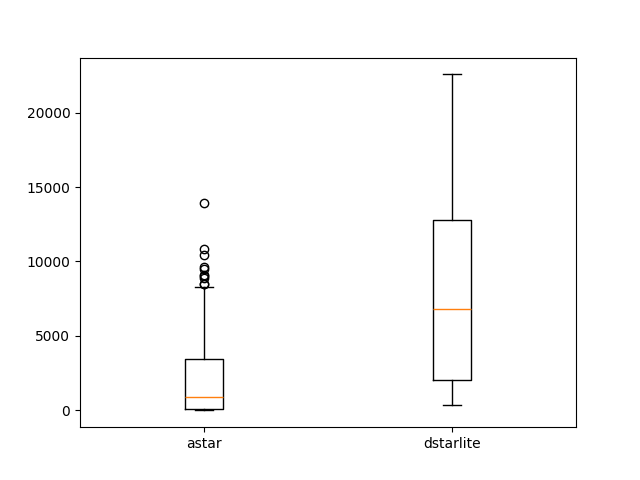
\includegraphics[width=\textwidth]{../plots/r50/Labyrinth-('dynswsffp', 'astar', 'dstarlite').png}
        \end{subfigure}
        \hfill
        \begin{subfigure}[b]{0.48\textwidth}
            \centering
            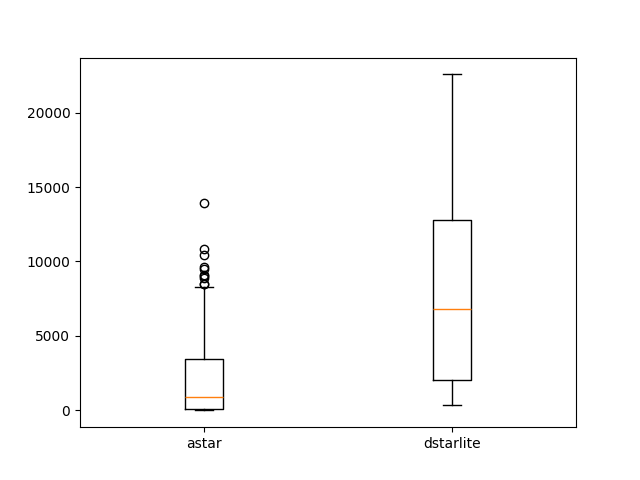
\includegraphics[width=\textwidth]{../plots/r50/Labyrinth-('astar', 'dstarlite').png}
        \end{subfigure}
        \caption{Labyrinth, большая видимость (радиус 50), производительность в ms}
        \label{fig: Labyrinth-r50}
    \end{figure}


    В-третьих, при большой видимости карты (иными словами, с увеличением радиуса видимости) алгоритм \dstarlite дает уже не такие впечатляющие результаты, существенно уступая в производительности \astar, см. Рис. \ref{fig: Labyrinth-r50}.


    \section{Заключение}
    Мы реализовали алгоритм \dstarlite, включащий в себя инкрементальность Dynamic SWSF-FP и использование эвристик, подобно \astar.
    Также мы провели его экспериментальное исследование, сравнив с вышеупомянутыми алгоритмами.
    Алгоритм показал себя исключительно хорошо в ситуациях малой видимости и на сложных картах.
    В других же ситуациях алгоритм давал результаты, которые в среднем несколько хуже, чем результаты \astar.

    \newpage
    \bibliography{main}
    \bibliographystyle{plain}

\end{document}